\begin{figure}[H]
	\centering
	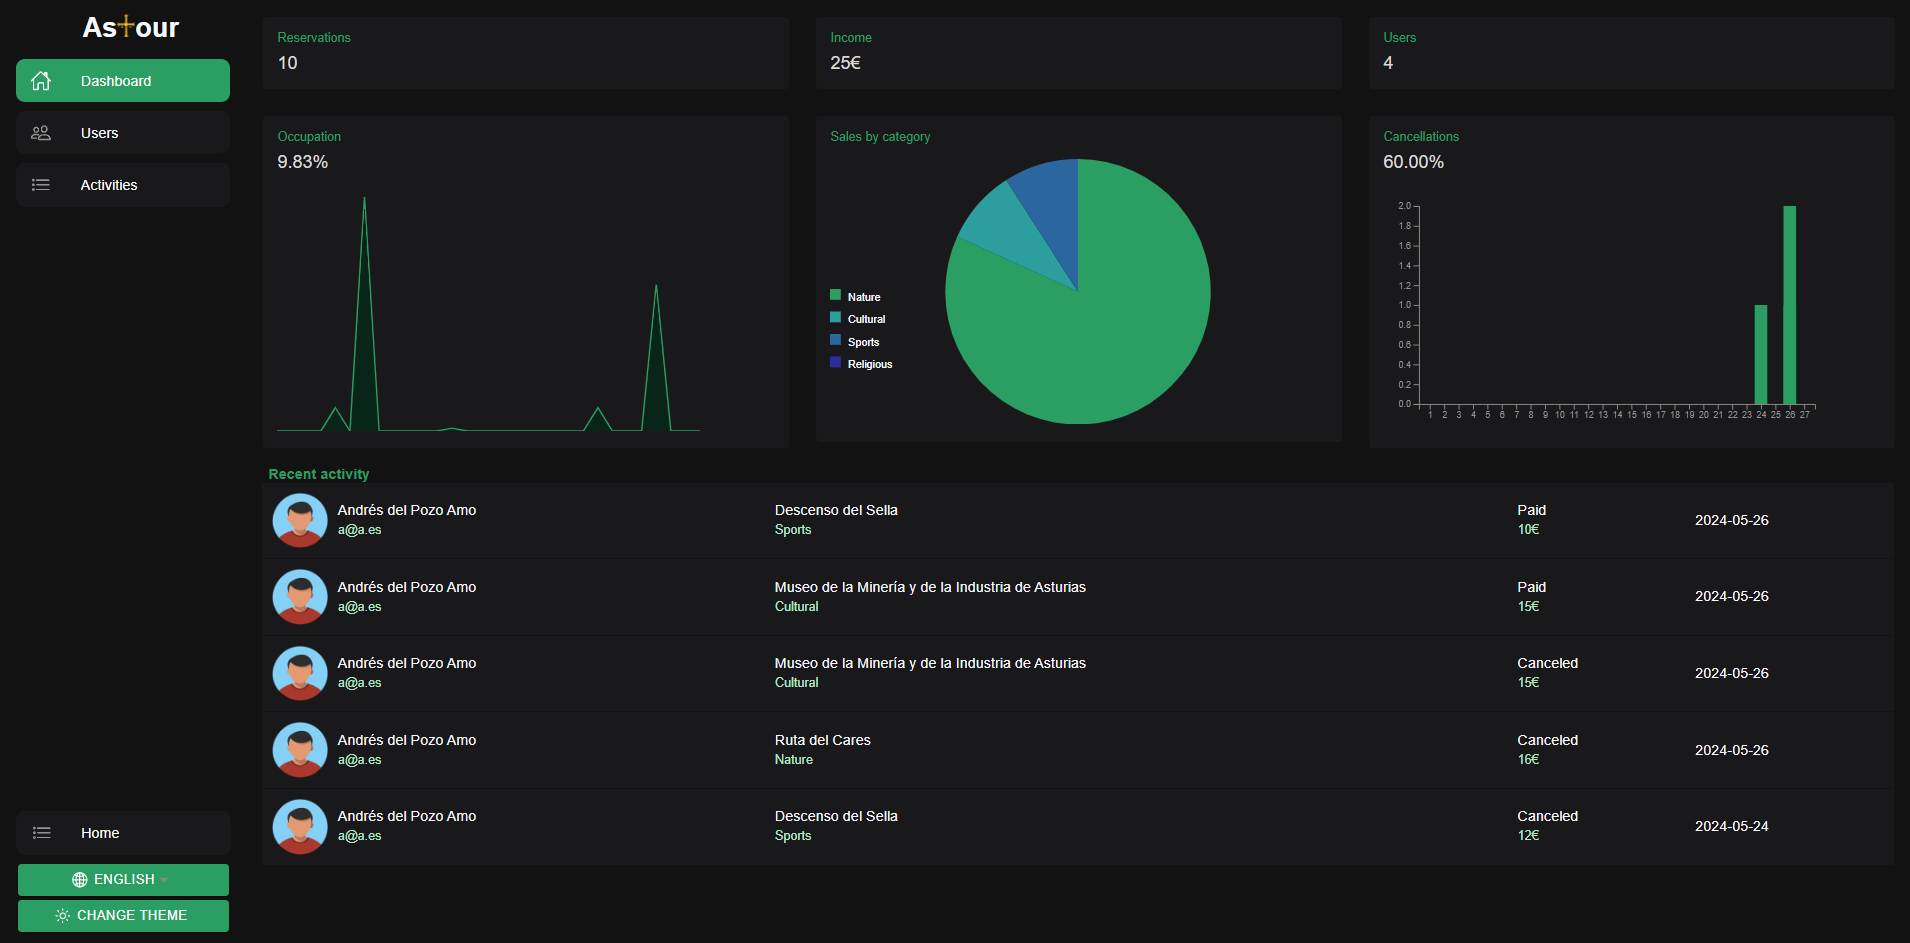
\includegraphics[width=0.8\textwidth]{6-DiseñoDelSistemaDeInformacion/RevisionInterfaces/Dashboard/panel-control.png}
	\caption{Dashboard - Panel de control}
\end{figure}


En el apartado “Usuarios” de la vista “Dashboard” se muestra una lista de los usuarios registrados en el sistema.
En la tabla se muestra el nombre, correo electrónico, el rol y las reservas realizadas de cada usuario.
Además, se incluye un botón para ver los detalles de cada usuario que nos llevará a la vista “Detalles de usuario” .

\begin{figure}[H]
	\centering
	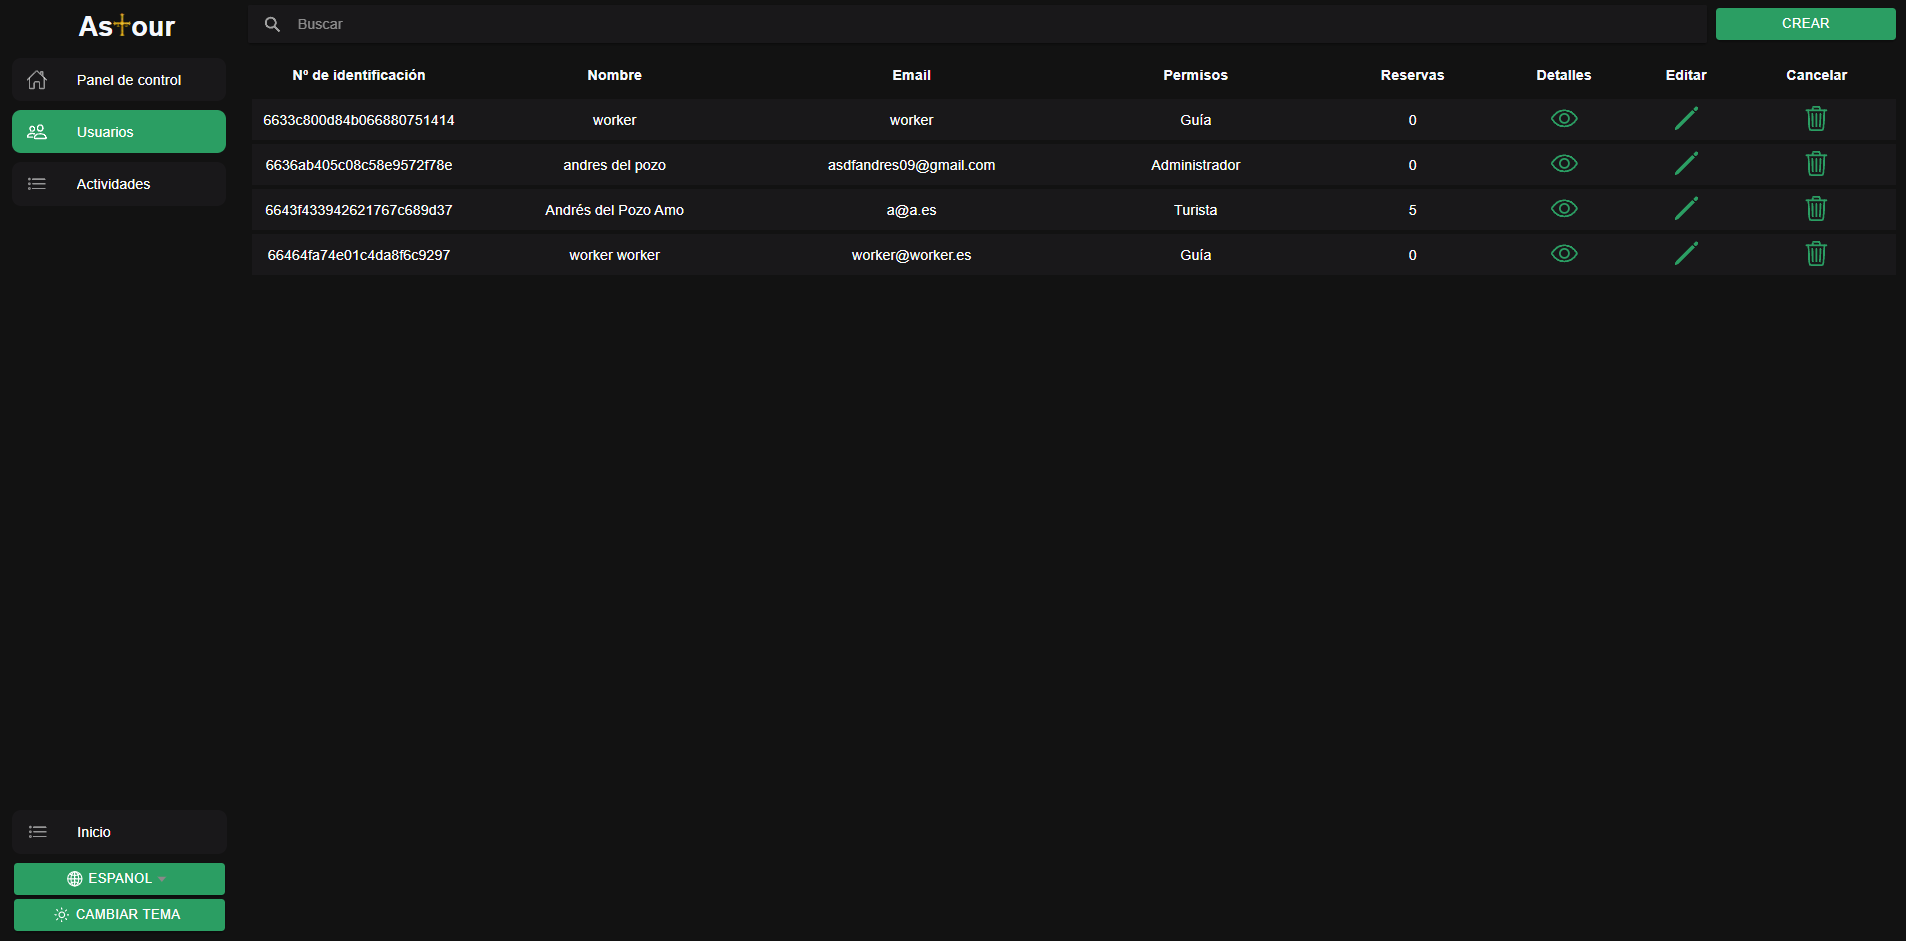
\includegraphics[width=0.8\textwidth]{6-DiseñoDelSistemaDeInformacion/RevisionInterfaces/Dashboard/usuarios.png}
	\caption{Dashboard - Lista de usuarios}
\end{figure}

\begin{figure}[H]
	\centering
	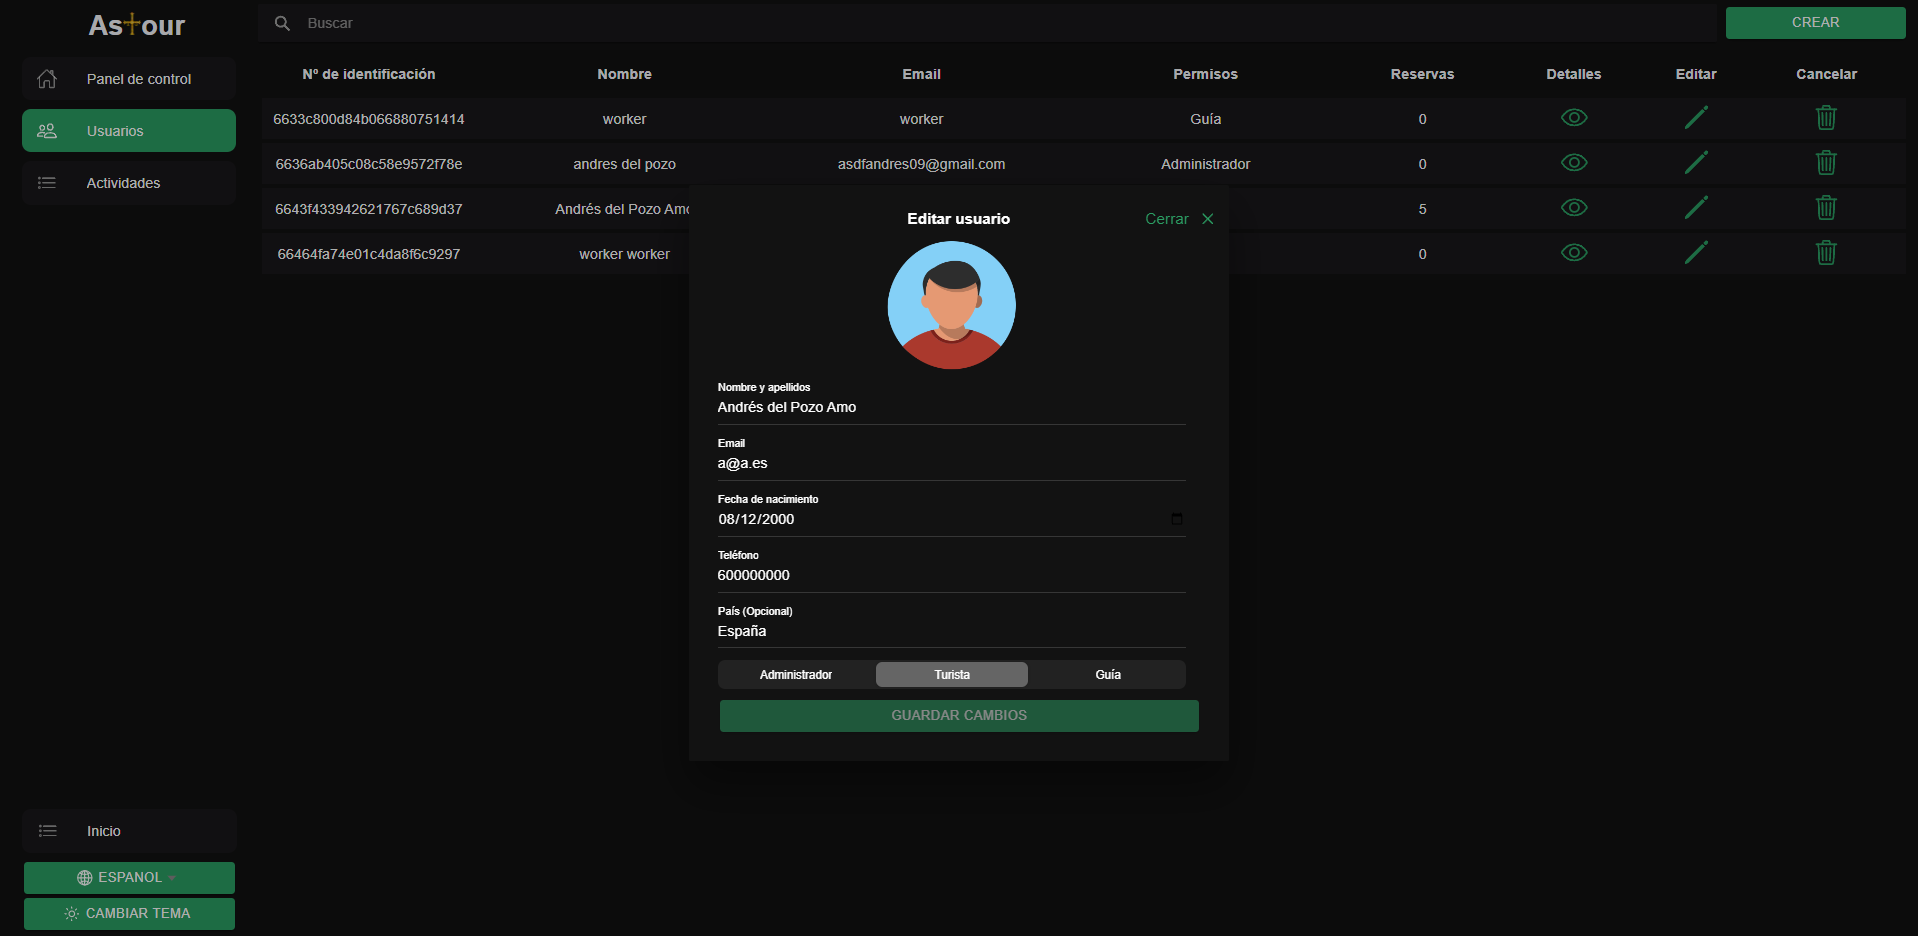
\includegraphics[width=0.8\textwidth]{6-DiseñoDelSistemaDeInformacion/RevisionInterfaces/Dashboard/usuarios-edit.png}
	\caption{Dashboard - Editar usuario}
\end{figure}

En el apartado “Actividades” de la vista “Dashboard” se muestra una lista de las actividades registradas en el sistema.
En la tabla se muestra el nombre, fecha de inicio, fecha de fin, lugar, descripción y el estado de cada actividad.
En caso de querer ver los eventos de una actividad, se puede hacer clic en la opción del menú lateral “Mostrar eventos” .

\begin{figure}[H]
	\centering
	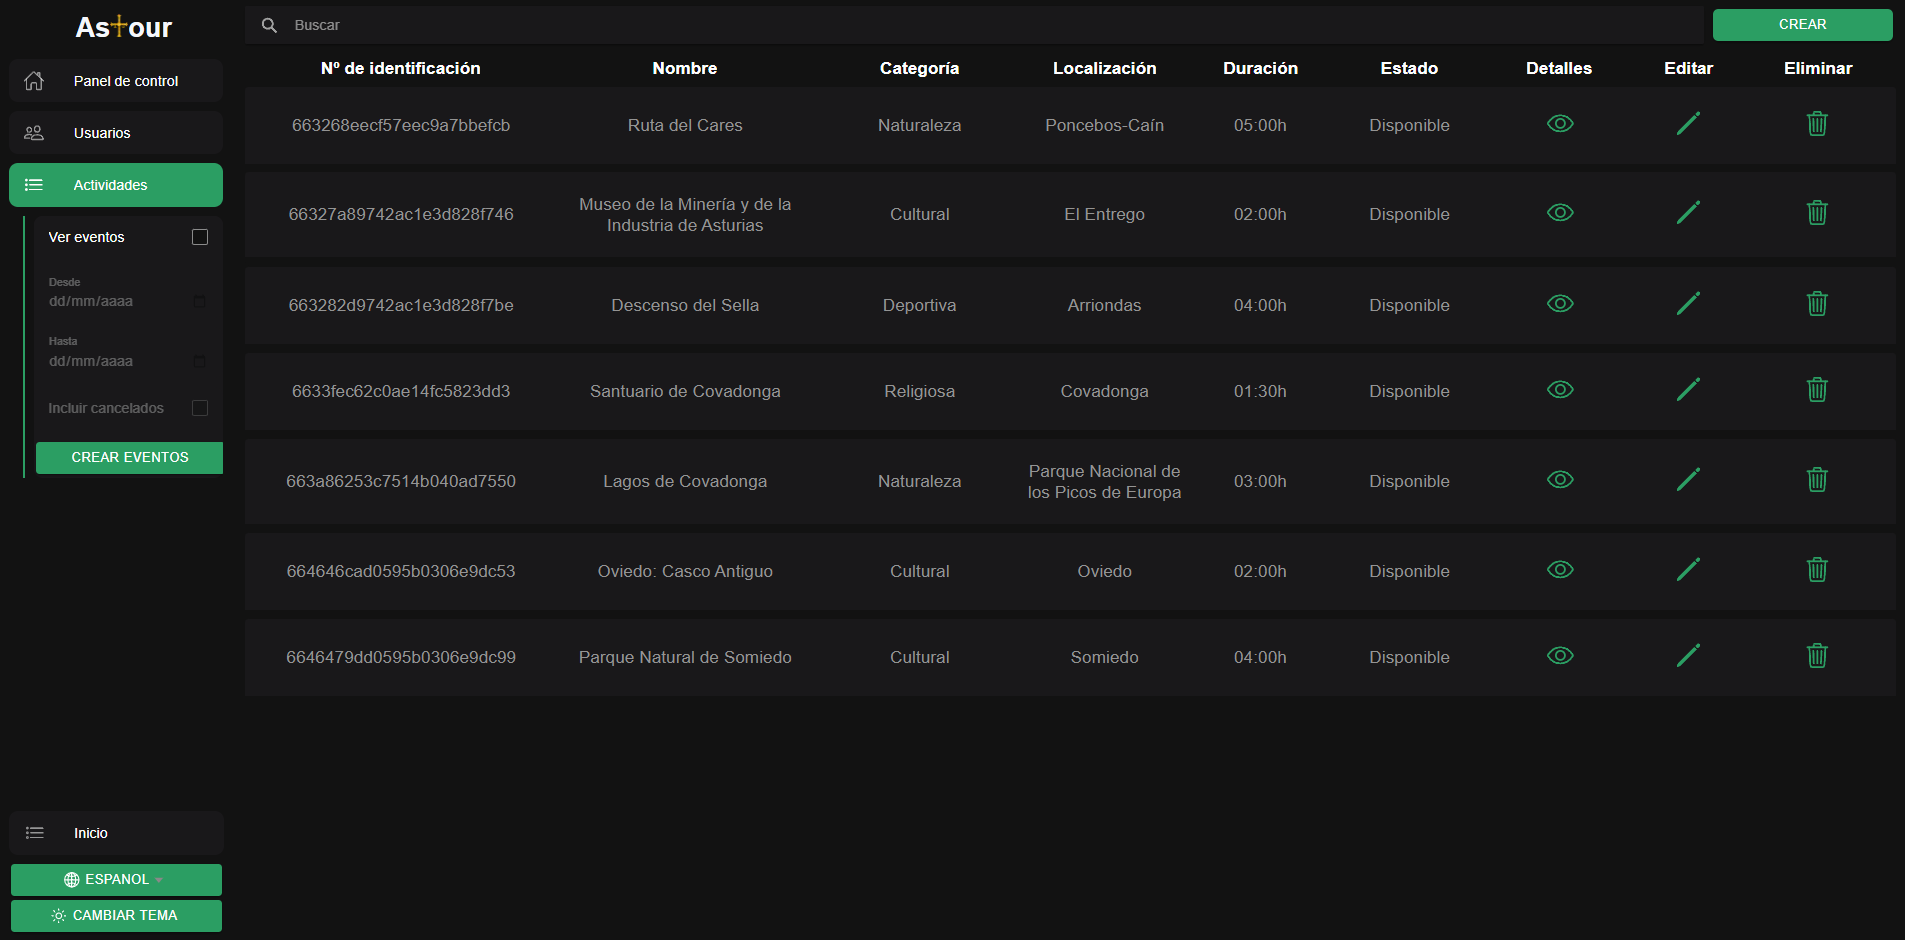
\includegraphics[width=0.8\textwidth]{6-DiseñoDelSistemaDeInformacion/RevisionInterfaces/Dashboard/actividades.png}
	\caption{Dashboard - Lista de actividades}
\end{figure}

\begin{figure}[H]
	\centering
	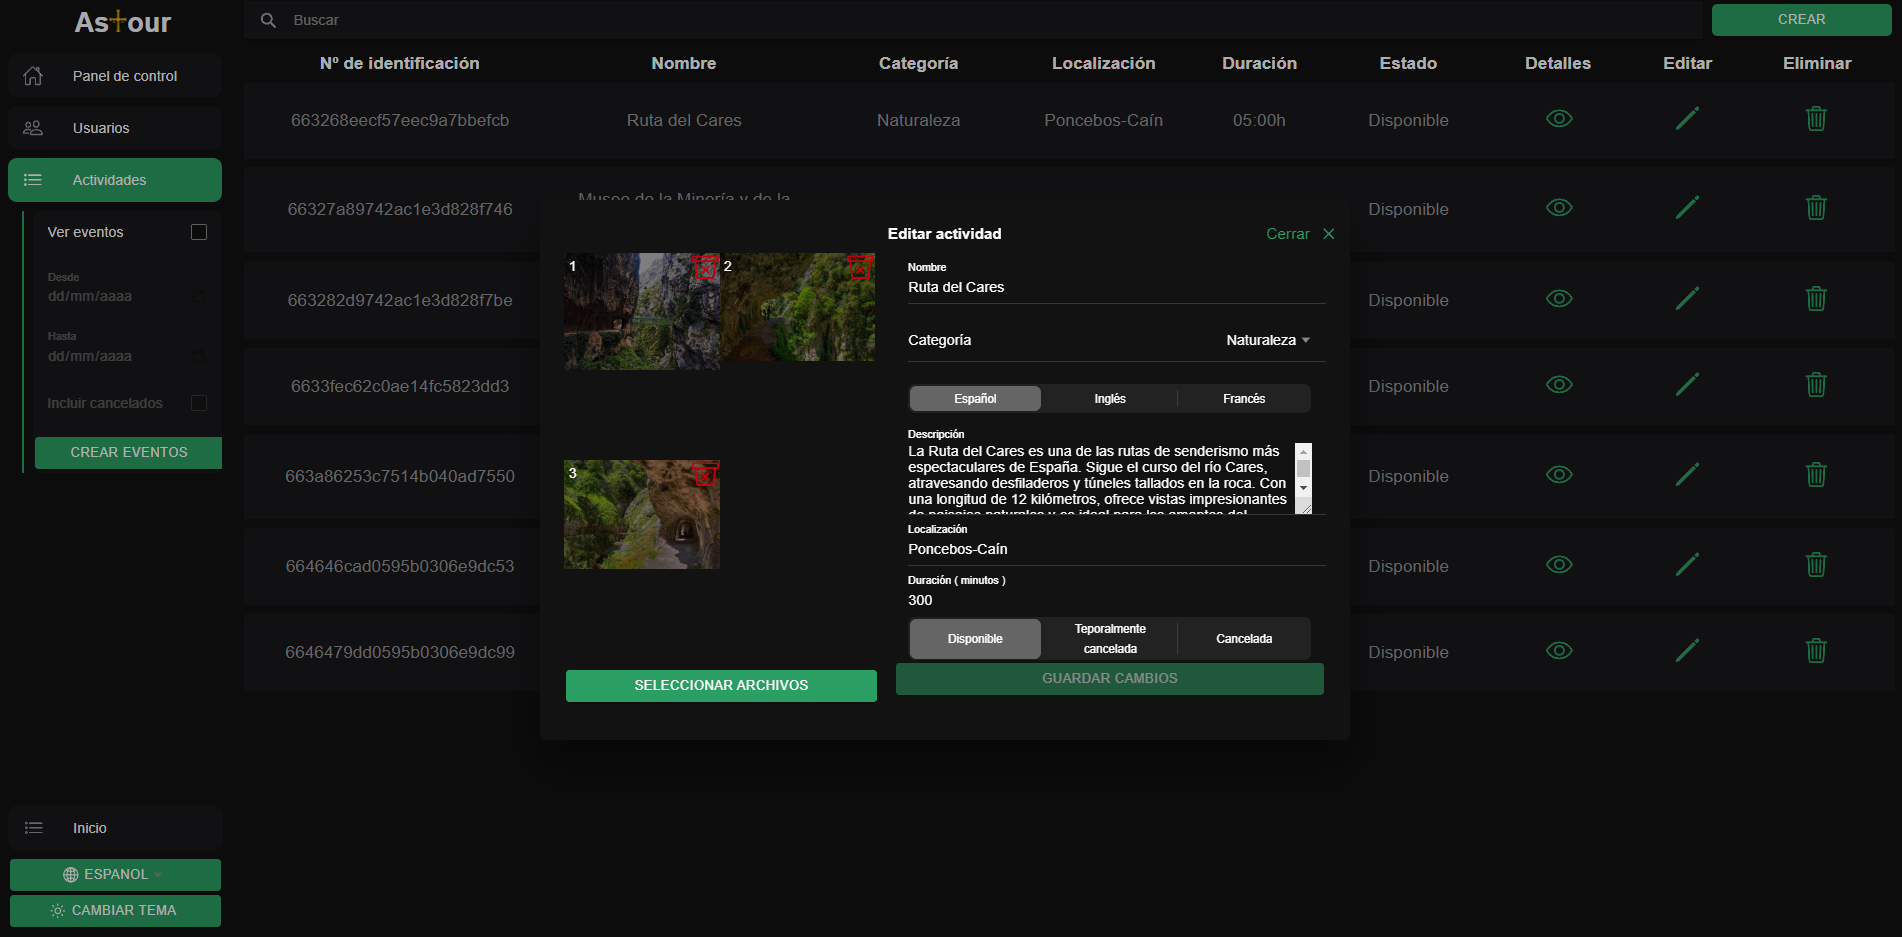
\includegraphics[width=0.8\textwidth]{6-DiseñoDelSistemaDeInformacion/RevisionInterfaces/Dashboard/actividades-edit.png}
	\caption{Dashboard - Editar actividad}
\end{figure}

\begin{figure}[H]
	\centering
	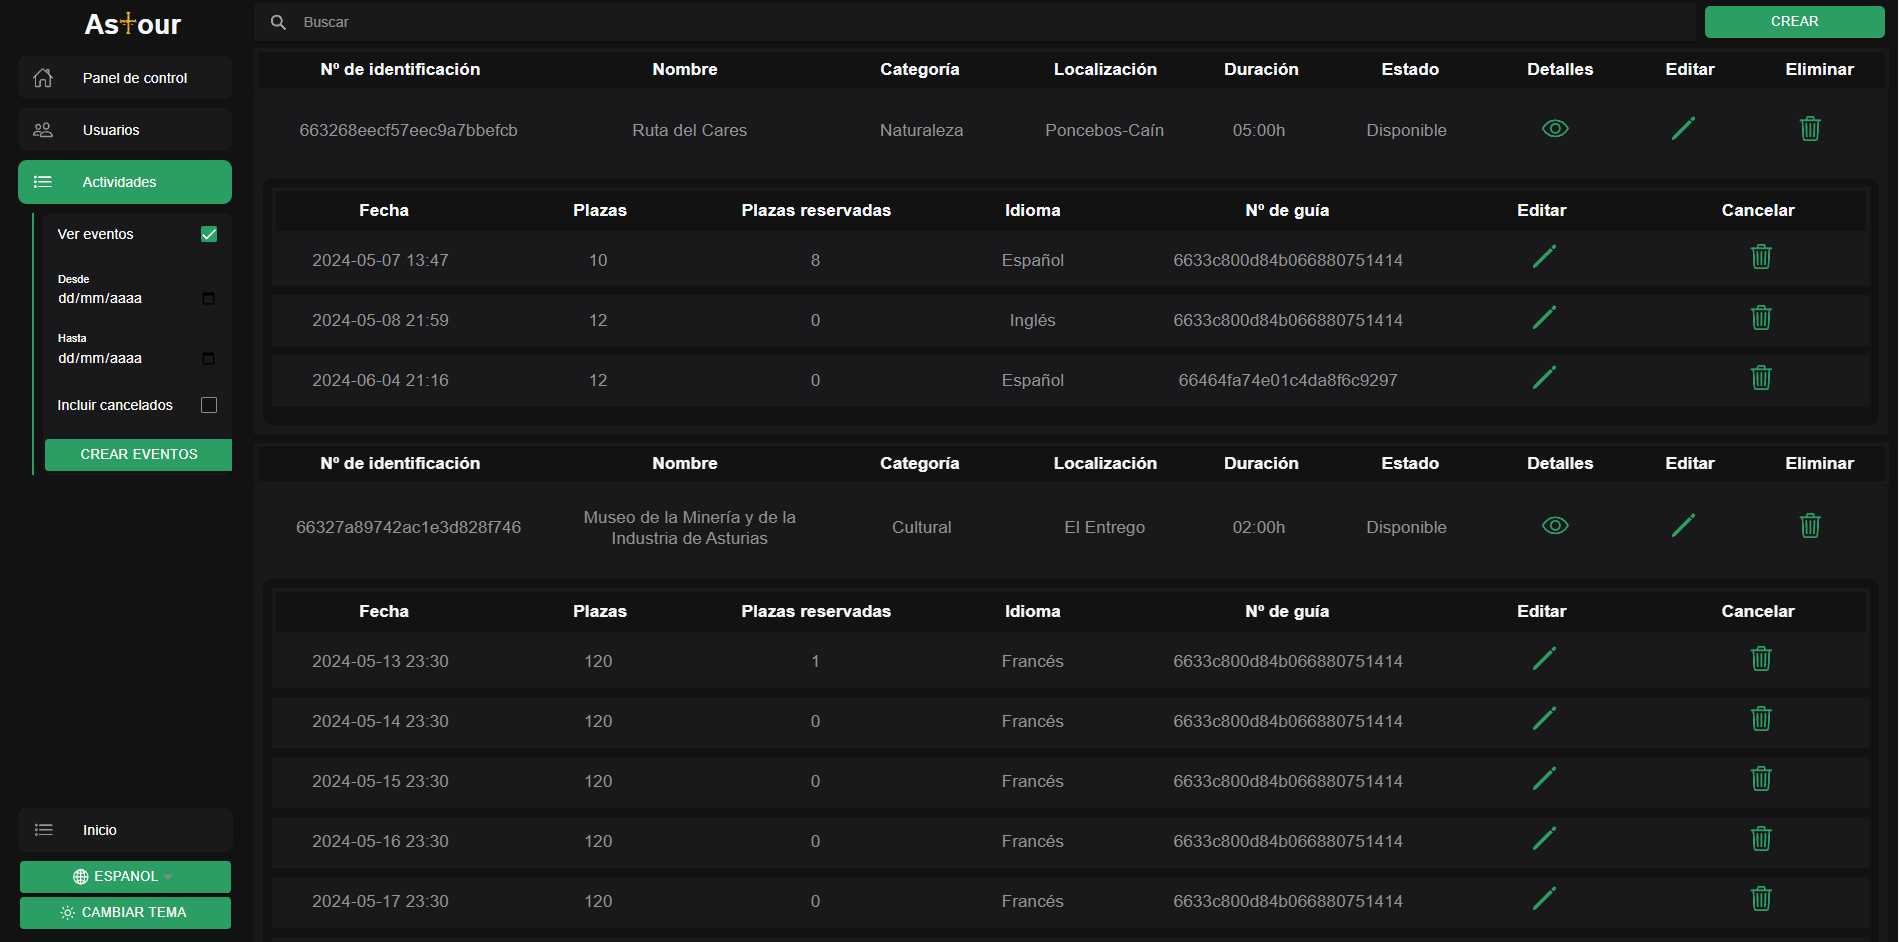
\includegraphics[width=0.8\textwidth]{6-DiseñoDelSistemaDeInformacion/RevisionInterfaces/Dashboard/eventos.png}
	\caption{Dashboard - Lista de actividades con eventos}
\end{figure}

\begin{figure}[H]
	\centering
	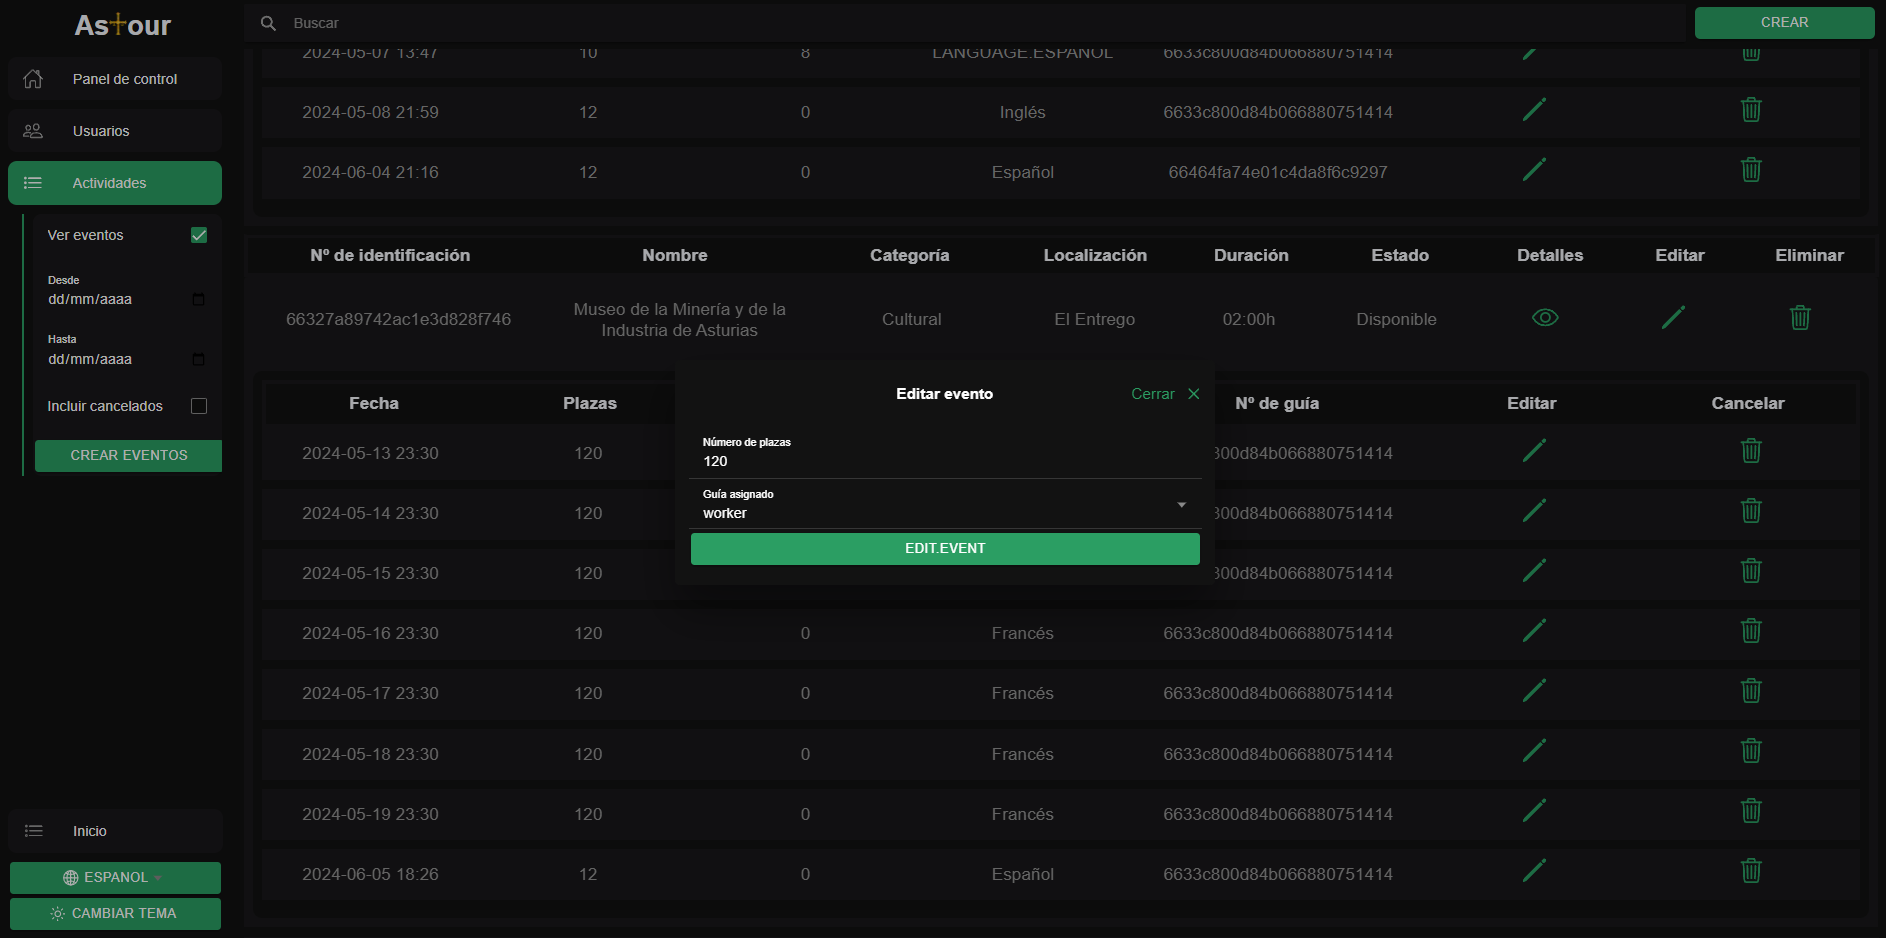
\includegraphics[width=0.8\textwidth]{6-DiseñoDelSistemaDeInformacion/RevisionInterfaces/Dashboard/eventos-edit.png}
	\caption{Dashboard - Editar evento}
\end{figure}

\subsubsection*{Detalles de usuario}
En la vista “Detalles de usuario” se muestra la información personal de un usuario, así como las reservas realizadas por el mismo.
Además, se incluye un botón para editar los datos del usuario y otro para cancelar una reserva.

\begin{figure}[H]
	\centering
	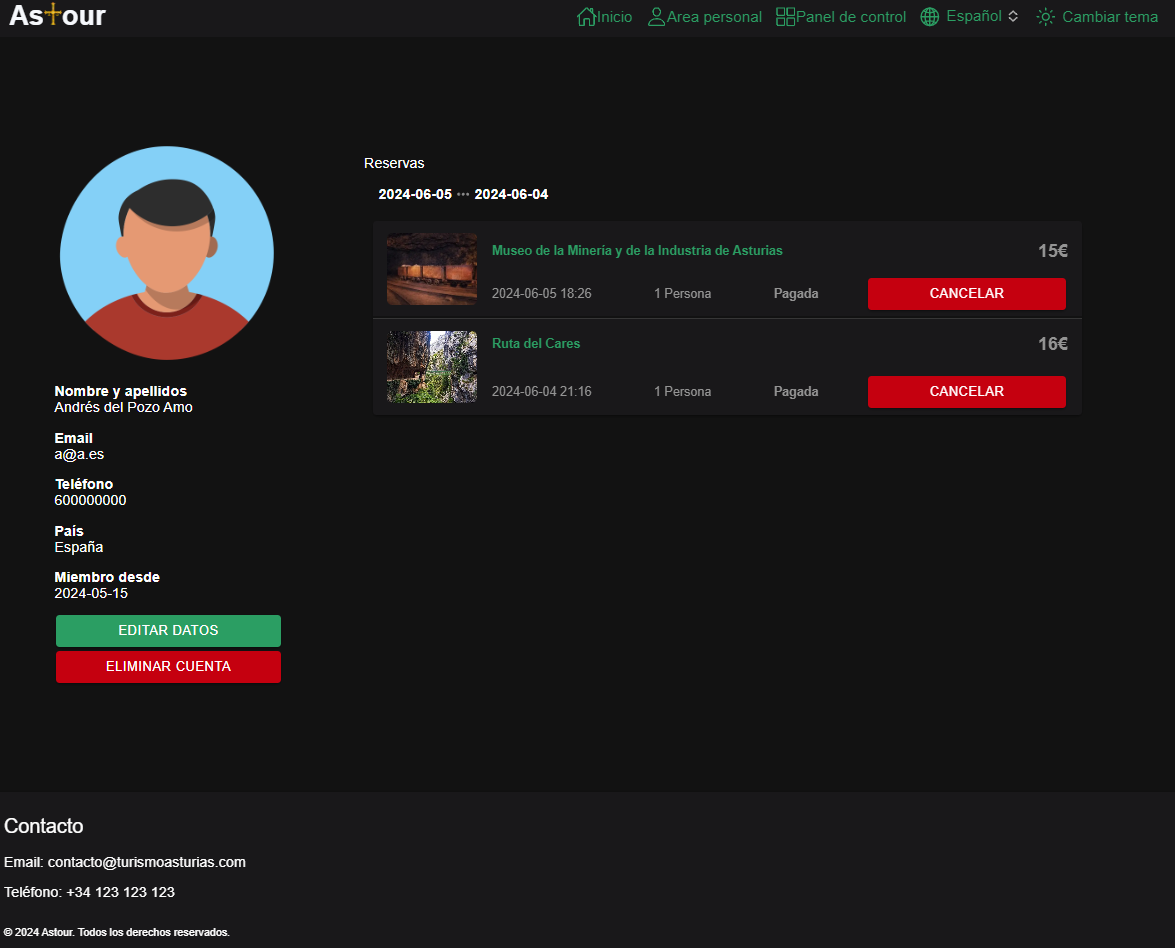
\includegraphics[width=0.8\textwidth]{6-DiseñoDelSistemaDeInformacion/RevisionInterfaces/Dashboard/detalles-usuario.png}
	\caption{Detalles de usuario}
\end{figure}

\begin{figure}[H]
	\centering
	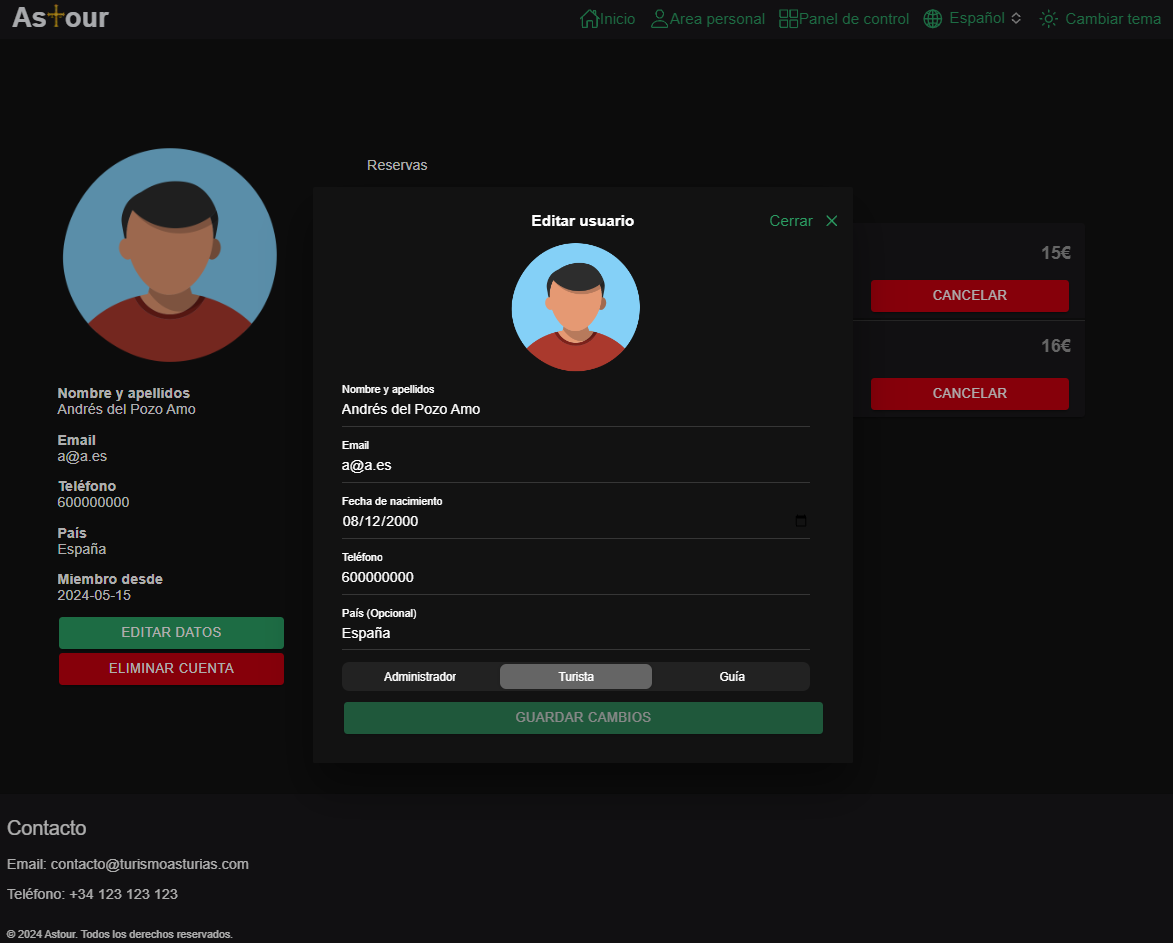
\includegraphics[width=0.8\textwidth]{6-DiseñoDelSistemaDeInformacion/RevisionInterfaces/Dashboard/detalles-usuario-editar.png}
	\caption{Detalles de usuario - Editar datos}
\end{figure}